\documentclass[12pt]{report}
\usepackage{amsmath}
\usepackage{graphicx}
\usepackage[colorlinks=true, linkcolor=black, citecolor=black, filecolor=black, urlcolor=black]{hyperref}
\usepackage{lipsum}
\usepackage{titlesec}
\usepackage{pdfpages}
\usepackage[utf8]{inputenc}
\title{Heat Production Management Project for Semester Project 2}
\author{Kacper Grzyb \and Sebestyen Deak \and Ignad Bozhinov \and Leonardo Gianola \and Levente Sohar}
\date{03-06-2024}

% Define a command to convert number section counting to alphabetical section counting
\makeatletter
\newcommand{\alphsection}{\@alph\c@section}
\makeatother

% Redefine the sectioning commands
\renewcommand{\thesection}{\thechapter\alphsection}
\titleformat{\section}
  {\normalfont\Large\bfseries}{\thesection}{1em}{}


\begin{document}
\maketitle

\tableofcontents

% Chapter 1
\chapter{Introduction}
Introduction chapter goes here

% Chapter 2
\chapter{Release Planning}
Release Planning chapter goes here

% Chapter 3
\chapter{Sprint Materials}
Sprint Planning Chapter goes here

\section{Sprint 1}

This should be the first pdf
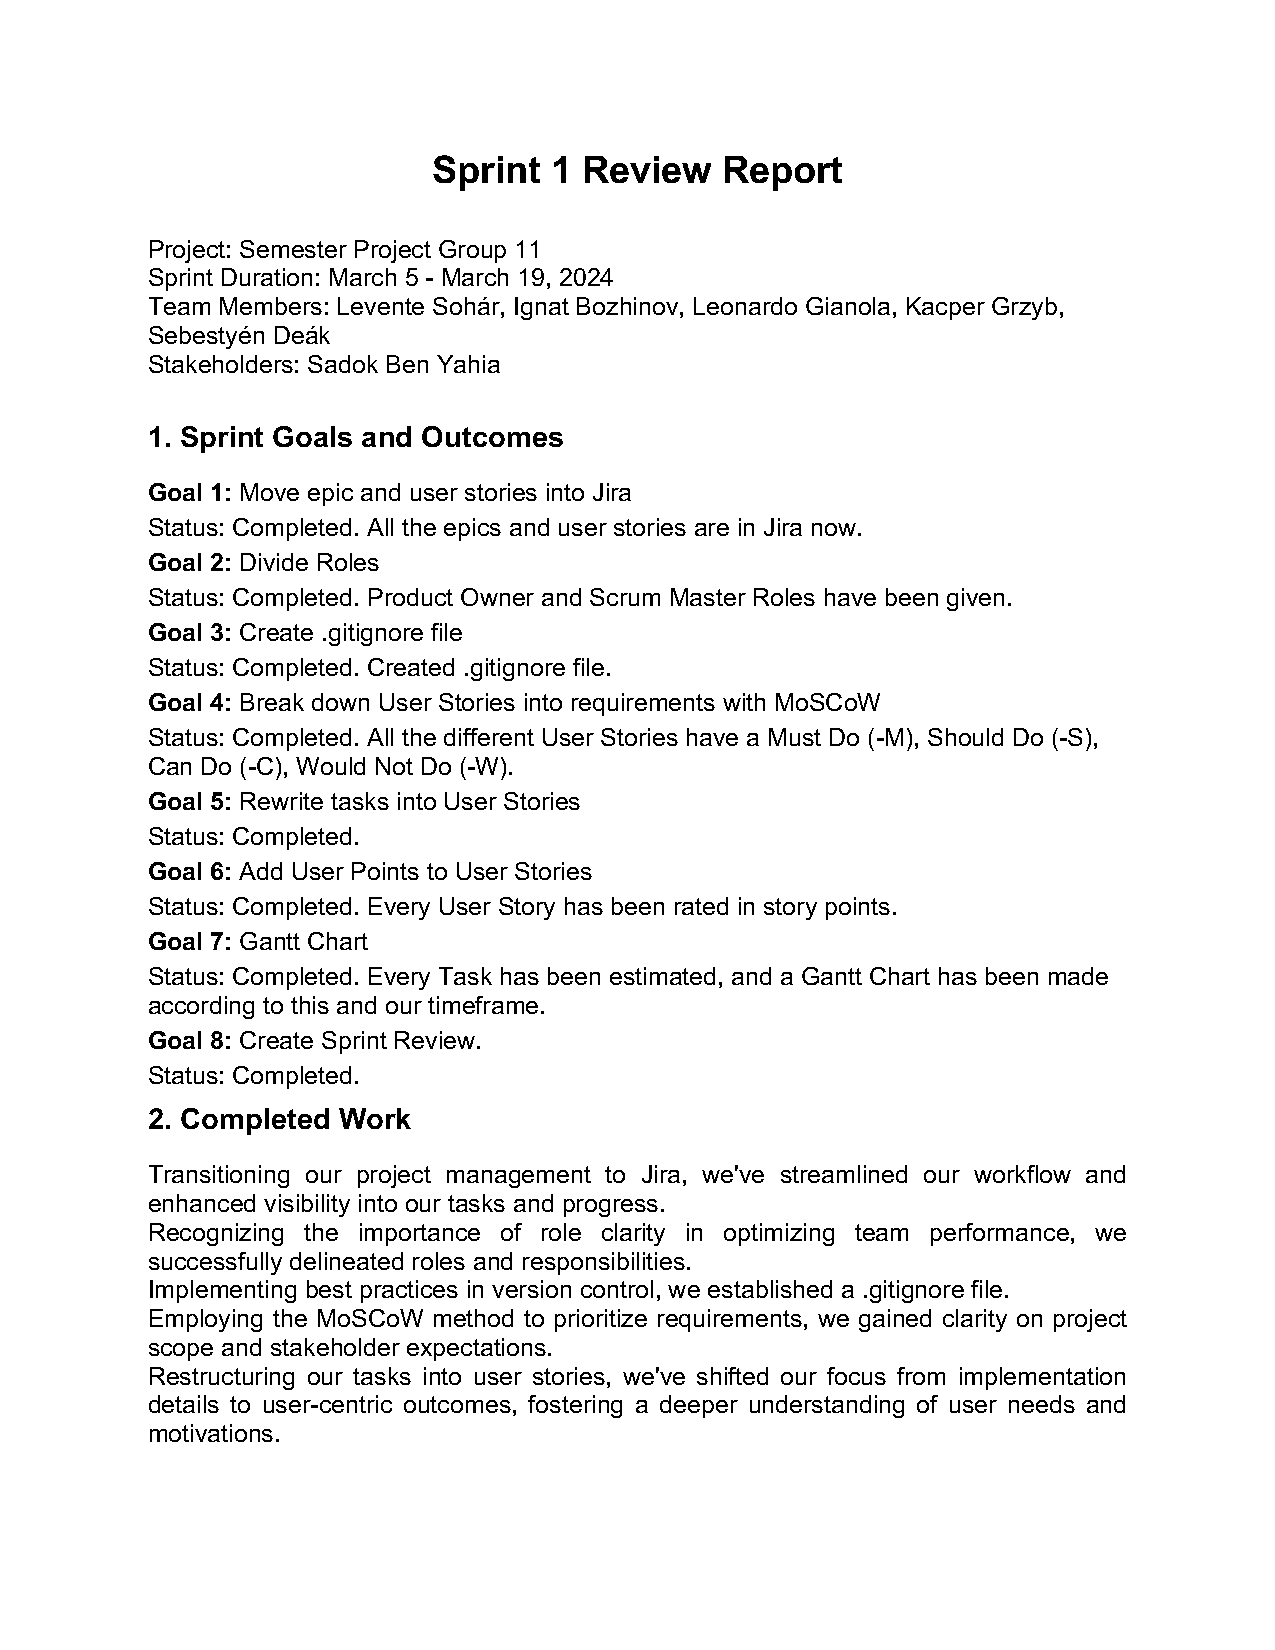
\includepdf[pages=-]{Resources/1-Sprint/Sprint-1-Review-Report.pdf}

This should be a ghant chart picture

\begin{figure}[h!]
    \centering
    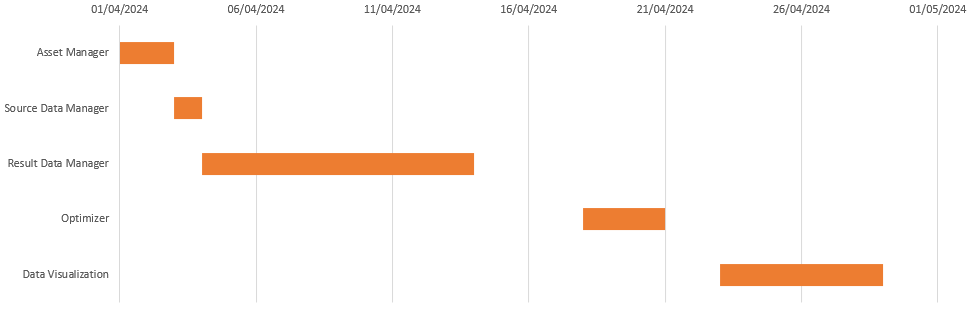
\includegraphics[width=0.5\textwidth]{Resources/1-Sprint/Gantt-Chart-Optimal.png}
    \caption{Optimal Ghant Chart}
    \label{fig:sample-image}
\end{figure}

\section{Sprint 2}
\section{Sprint 3}
\section{Sprint 4}


% Chapter 4
\chapter{Technical Details}
Technical Details Chapter goes here

% Chapter 4a
\section{Design and UML Diagrams}
Design and UML Diagrams yapping goes here

% Chapter 4b
\section{Simple Design}
Simple design yapping goes here

% Chapter 4c
\section{Incremental Design}
Incremental Design yapping goes here

% Chapter 4d
\section{Refactoring}
Refactoring yapping goes here

% Chapter 4e
\section{Test-Driven Development}
Test-Driven Development yapping goes here

% Chapter 4f
\section{Unit Testing}
Unit Testing yapping goes here

% Chapter 4g
\section{Pair Programming}
Pair Programming yapping goes here

% Chapter 4h
\section{Code Review}
Code Review yapping goes here

% Chapter 5
\chapter{Conclusion and Group's Reflections}
Conclusion chapter goes here

% Chapter 5a
\section{Working on a common project with other groups}
5a yapping goes here

% Chapter 5b
\section{What went well and not so well with the group's specific set of tasks}
5b yapping goes here

% Chapter 5c
\section{Specific contributions of each team member}
5c yapping goes here

\section{Future actions to prevent problems and difficulties faced during the project}
5d yapping goes here


\end{document}